\documentclass{standalone}
\usepackage{tikz}
\usetikzlibrary{patterns, positioning}

\begin{document}
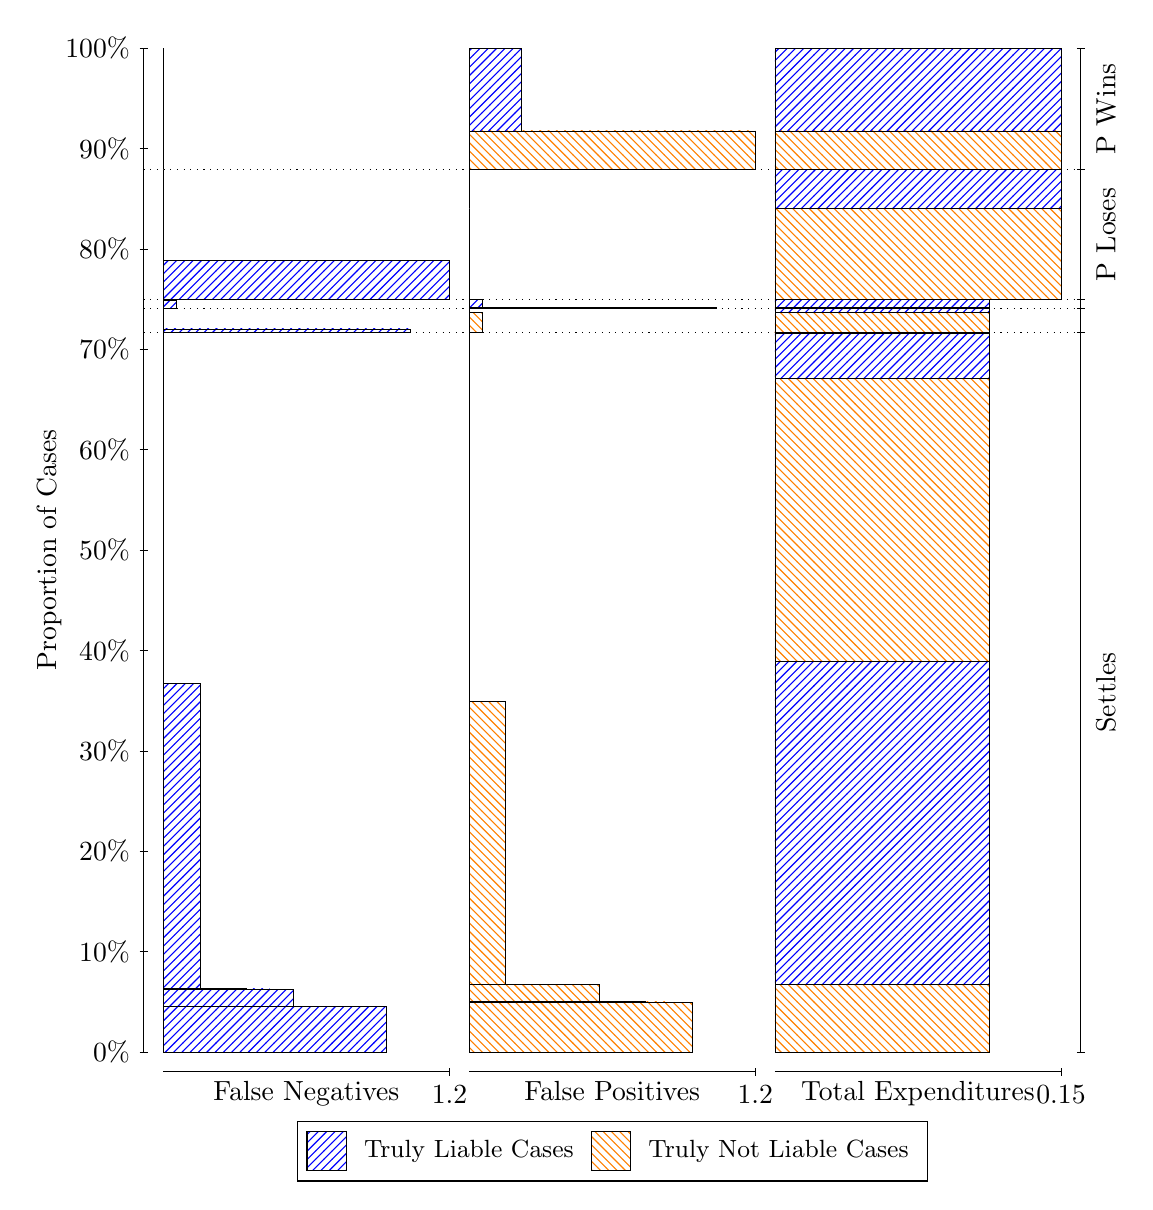
\begin{tikzpicture}
\draw[black, very thin] (1.5,1.75) -- (1.5,14.5);
\node[rotate=90, anchor=center] at (0.3, 8.125) {Proportion of Cases};
\draw[black, very thin] (1.45,1.75) -- (1.55,1.75);
\node[anchor=east] at (1.45, 1.75) {0\%};
\draw[black, very thin] (1.45,3.025) -- (1.55,3.025);
\node[anchor=east] at (1.45, 3.025) {10\%};
\draw[black, very thin] (1.45,4.3) -- (1.55,4.3);
\node[anchor=east] at (1.45, 4.3) {20\%};
\draw[black, very thin] (1.45,5.575) -- (1.55,5.575);
\node[anchor=east] at (1.45, 5.575) {30\%};
\draw[black, very thin] (1.45,6.85) -- (1.55,6.85);
\node[anchor=east] at (1.45, 6.85) {40\%};
\draw[black, very thin] (1.45,8.125) -- (1.55,8.125);
\node[anchor=east] at (1.45, 8.125) {50\%};
\draw[black, very thin] (1.45,9.4) -- (1.55,9.4);
\node[anchor=east] at (1.45, 9.4) {60\%};
\draw[black, very thin] (1.45,10.675) -- (1.55,10.675);
\node[anchor=east] at (1.45, 10.675) {70\%};
\draw[black, very thin] (1.45,11.95) -- (1.55,11.95);
\node[anchor=east] at (1.45, 11.95) {80\%};
\draw[black, very thin] (1.45,13.225) -- (1.55,13.225);
\node[anchor=east] at (1.45, 13.225) {90\%};
\draw[black, very thin] (1.45,14.5) -- (1.55,14.5);
\node[anchor=east] at (1.45, 14.5) {100\%};

\draw[black, very thin] (13.4,1.75) -- (13.4,14.5);
\draw[black, very thin] (13.35,1.75) -- (13.45,1.75);
\node[anchor=west] at (13.35, 1.75) {};
\draw[black, very thin] (13.35,10.885) -- (13.45,10.885);
\node[anchor=west] at (13.35, 10.885) {};
\draw[black, very thin] (13.35,11.191) -- (13.45,11.191);
\node[anchor=west] at (13.35, 11.191) {};
\draw[black, very thin] (13.35,11.305) -- (13.45,11.305);
\node[anchor=west] at (13.35, 11.305) {};
\draw[black, very thin] (13.35,12.955) -- (13.45,12.955);
\node[anchor=west] at (13.35, 12.955) {};
\draw[black, very thin] (13.35,14.5) -- (13.45,14.5);
\node[anchor=west] at (13.35, 14.5) {};

\draw[black, very thin, pattern color=blue, pattern=north east lines] (1.75,1.75) rectangle (4.5862,2.3277);
\draw[black, very thin, pattern color=blue, pattern=north east lines] (1.75,2.3277) rectangle (4.2896,2.3285);
\draw[black, very thin, pattern color=blue, pattern=north east lines] (1.75,2.3285) rectangle (3.993,2.3294);
\draw[black, very thin, pattern color=blue, pattern=north east lines] (1.75,2.3294) rectangle (3.6964,2.3302);
\draw[black, very thin, pattern color=blue, pattern=north east lines] (1.75,2.3302) rectangle (3.3998,2.5447);
\draw[black, very thin, pattern color=blue, pattern=north east lines] (1.75,2.5447) rectangle (3.1032,2.55);
\draw[black, very thin, pattern color=blue, pattern=north east lines] (1.75,2.55) rectangle (2.8066,2.5552);
\draw[black, very thin, pattern color=blue, pattern=north east lines] (1.75,2.5552) rectangle (2.51,2.5605);
\draw[black, very thin, pattern color=blue, pattern=north east lines] (1.75,2.5605) rectangle (2.2134,6.4293);
\draw[black, very thin, pattern color=orange, pattern=north west lines] (1.75,6.4293) rectangle (1.75,10.885);
\draw[black, very thin, pattern color=blue, pattern=north east lines] (1.75,10.885) rectangle (4.8828,10.932);
\draw[black, very thin, pattern color=orange, pattern=north west lines] (1.75,10.932) rectangle (1.75,11.191);
\draw[black, very thin, pattern color=blue, pattern=north east lines] (1.75,11.191) rectangle (1.9168,11.294);
\draw[black, very thin, pattern color=orange, pattern=north west lines] (1.75,11.294) rectangle (1.75,11.305);
\draw[black, very thin, pattern color=blue, pattern=north east lines] (1.75,11.305) rectangle (5.3833,11.8);
\draw[black, very thin, pattern color=orange, pattern=north west lines] (1.75,11.8) rectangle (1.75,12.955);
\draw[black, very thin, pattern color=orange, pattern=north west lines] (1.75,12.955) rectangle (1.75,13.449);
\draw[black, very thin, pattern color=blue, pattern=north east lines] (1.75,13.449) rectangle (1.75,14.5);
\draw[black, very thin, pattern color=orange, pattern=north west lines] (5.6333,1.75) rectangle (8.4696,2.3801);
\draw[black, very thin, pattern color=orange, pattern=north west lines] (5.6333,2.3801) rectangle (8.173,2.3855);
\draw[black, very thin, pattern color=orange, pattern=north west lines] (5.6333,2.3855) rectangle (7.8764,2.3909);
\draw[black, very thin, pattern color=orange, pattern=north west lines] (5.6333,2.3909) rectangle (7.5798,2.3963);
\draw[black, very thin, pattern color=orange, pattern=north west lines] (5.6333,2.3963) rectangle (7.2832,2.6119);
\draw[black, very thin, pattern color=orange, pattern=north west lines] (5.6333,2.6119) rectangle (6.9866,2.6119);
\draw[black, very thin, pattern color=orange, pattern=north west lines] (5.6333,2.6119) rectangle (6.9866,2.6124);
\draw[black, very thin, pattern color=orange, pattern=north west lines] (5.6333,2.6124) rectangle (6.69,2.6128);
\draw[black, very thin, pattern color=orange, pattern=north west lines] (5.6333,2.6128) rectangle (6.3934,2.6132);
\draw[black, very thin, pattern color=orange, pattern=north west lines] (5.6333,2.6132) rectangle (6.0968,6.2058);
\draw[black, very thin, pattern color=blue, pattern=north east lines] (5.6333,6.2058) rectangle (5.6333,10.885);
\draw[black, very thin, pattern color=orange, pattern=north west lines] (5.6333,10.885) rectangle (5.8002,11.144);
\draw[black, very thin, pattern color=blue, pattern=north east lines] (5.6333,11.144) rectangle (5.6333,11.191);
\draw[black, very thin, pattern color=orange, pattern=north west lines] (5.6333,11.191) rectangle (8.7662,11.202);
\draw[black, very thin, pattern color=blue, pattern=north east lines] (5.6333,11.202) rectangle (5.8002,11.305);
\draw[black, very thin, pattern color=orange, pattern=north west lines] (5.6333,11.305) rectangle (5.6333,12.459);
\draw[black, very thin, pattern color=blue, pattern=north east lines] (5.6333,12.459) rectangle (5.6333,12.955);
\draw[black, very thin, pattern color=orange, pattern=north west lines] (5.6333,12.955) rectangle (9.2667,13.449);
\draw[black, very thin, pattern color=blue, pattern=north east lines] (5.6333,13.449) rectangle (6.3007,14.5);
\draw[black, very thin, pattern color=orange, pattern=north west lines] (9.5167,1.75) rectangle (12.242,2.6119);
\draw[black, very thin, pattern color=blue, pattern=north east lines] (9.5167,2.6119) rectangle (12.242,6.711);
\draw[black, very thin, pattern color=orange, pattern=north west lines] (9.5167,6.711) rectangle (12.242,10.304);
\draw[black, very thin, pattern color=blue, pattern=north east lines] (9.5167,10.304) rectangle (12.242,10.881);
\draw[black, very thin, pattern color=orange, pattern=north west lines] (9.5167,10.881) rectangle (12.242,10.882);
\draw[black, very thin, pattern color=blue, pattern=north east lines] (9.5167,10.882) rectangle (12.242,10.884);
\draw[black, very thin, pattern color=orange, pattern=north west lines] (9.5167,10.884) rectangle (12.242,10.884);
\draw[black, very thin, pattern color=blue, pattern=north east lines] (9.5167,10.884) rectangle (12.242,10.885);
\draw[black, very thin, pattern color=orange, pattern=north west lines] (9.5167,10.885) rectangle (12.242,11.144);
\draw[black, very thin, pattern color=blue, pattern=north east lines] (9.5167,11.144) rectangle (12.242,11.191);
\draw[black, very thin, pattern color=orange, pattern=north west lines] (9.5167,11.191) rectangle (12.242,11.202);
\draw[black, very thin, pattern color=blue, pattern=north east lines] (9.5167,11.202) rectangle (12.242,11.305);
\draw[black, very thin, pattern color=orange, pattern=north west lines] (9.5167,11.305) rectangle (13.15,12.459);
\draw[black, very thin, pattern color=blue, pattern=north east lines] (9.5167,12.459) rectangle (13.15,12.955);
\draw[black, very thin, pattern color=orange, pattern=north west lines] (9.5167,12.955) rectangle (13.15,13.449);
\draw[black, very thin, pattern color=blue, pattern=north east lines] (9.5167,13.449) rectangle (13.15,14.5);
\draw[black, dotted] (1.5,10.885) -- (13.4,10.885);
\draw[black, dotted] (1.5,11.191) -- (13.4,11.191);
\draw[black, dotted] (1.5,11.305) -- (13.4,11.305);
\draw[black, dotted] (1.5,12.955) -- (13.4,12.955);
\draw[black, very thin] (1.75,1.5) -- (5.3833,1.5);
\node[anchor=north] at (3.5667, 1.5) {False Negatives};
\draw[black, very thin] (5.3833,1.45) -- (5.3833,1.55);
\node[anchor=north] at (5.3833, 1.45) {1.2};

\draw[black, very thin] (5.6333,1.5) -- (9.2667,1.5);
\node[anchor=north] at (7.45, 1.5) {False Positives};
\draw[black, very thin] (9.2667,1.45) -- (9.2667,1.55);
\node[anchor=north] at (9.2667, 1.45) {1.2};

\draw[black, very thin] (9.5167,1.5) -- (13.15,1.5);
\node[anchor=north] at (11.333, 1.5) {Total Expenditures};
\draw[black, very thin] (13.15,1.45) -- (13.15,1.55);
\node[anchor=north] at (13.15, 1.45) {0.15};

\node[black, centered, rotate=90] at (13.72, 6.3175) {Settles};


\node[black, centered, rotate=90] at (13.72, 12.13) {P Loses};
\node[black, centered, rotate=90] at (13.72, 13.727) {P Wins};

\draw (7.449999999999999,1.5) node[draw=none] (baseCoordinate) {};
\begin{scope}[align=center]
        \matrix[scale=0.5, draw=black, below=0.5cm of baseCoordinate, nodes={draw}, column sep=0.1cm]{
            \node[rectangle, draw, minimum width=0.5cm, minimum height=0.5cm, pattern=north east lines, pattern color=blue] {}; &
            \node[draw=none, font=\small] (B) {Truly Liable Cases}; &
            \node[rectangle, draw, minimum width=0.5cm, minimum height=0.5cm, pattern=north west lines, pattern color=orange] {}; &
            \node[draw=none, font=\small] (B) {Truly Not Liable Cases}; \\
            };
\end{scope}

\end{tikzpicture}
\end{document}